\section{Automatic Accuracy Evaluation}\label{appendix:autoeval}

To verify the efficacy of automatic accuracy evaluation by \GPTName and \LLaMATwoName, we compare their judgements' alignment with human annotations.
Specifically, we first sample 80 (question, response) pairs for each (model, dataset), resulting in 720 samples in total.
We then manually compare each sample's response with the reference answer, and decide if the generated response is correct (given the context if any).
Then, we retrieve the ratings on these 720 samples from \GPTName and \LLaMATwoName, and find the thresholds that result in the highest agreement.
The resulting accuracy-threshold relation is illustrated in \cref{fig:appendix:autoeval_thres}.
From the results, we chose 0.2 as the threshold for \LLaMATwoName and 0.6 for \GPTName.
In other words, denote the rating from \LLaMATwoName on a generated response $\predSeq$ as $r_{llama2}(\predSeq)$, then $\text{acc}_{llama2}(\predSeq) = \mathbbm{1}\{r_{llama2}(\predSeq) \geq 0.2\}$.
Note that we found 20 out of the 720 samples hard to decide during our manual annotation process, usually due to incorrect reference answers or intrinsic ambiguity in the questions. 
We ignore them during the computation of \cref{fig:appendix:autoeval_thres}.

\def \FigAppendixAEThres{
\begin{figure}[ht]
\centering
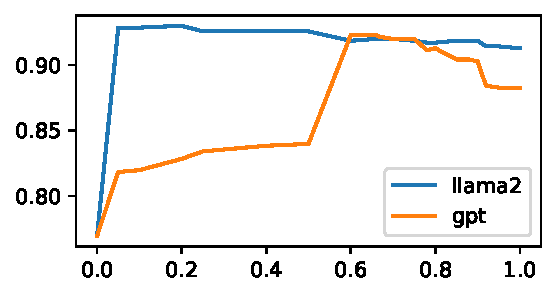
\includegraphics[width=0.4\textwidth]{Figures/appendix_eval_thres.pdf}
\caption{
Agreement with human annotation with different thresholds over all 720 samples.
}
\label{fig:appendix:autoeval_thres}
\end{figure}
}
\FigAppendixAEThres

